\documentclass[12pt, a4paper]{report}
\usepackage[italian]{babel}
\usepackage{float}
\usepackage{graphicx}
\usepackage{hyperref}

\renewcommand{\familydefault}{\sfdefault}


\begin{document}
    \title{
        
\includegraphics[width=0.4\textwidth]{assets/logo.png}\\
        [1cm]CucinAssistant: Guida all'utilizzo\\
        \large aggiornata alla versione \emph{6.0 (Zucchina)}
    }
    \author{Gianluca Parri}
    \date{\today}
    \maketitle



    \tableofcontents
    \vfill
    \noindent Per segnalare errori o suggerimenti potete scrivere a \href{mailto:info@cucinassistant.com}{\mbox{info@cucinassistant.com}}.



    \chapter{Novità}
    
    Le modifiche apportate a CucinAssistant dall'ultima versione (\emph{5.0, Patata}) sono qui riassunte:

    \begin{itemize}
        \item Interfaccia utente multilingua [\ref{changelang}]
        \item Nuova sezione ricette [\ref{recipes}]
        \item Aggiunto un pulsante per poter inserire articoli in dispensa in diverse sezioni
        \item Possibilità di impostare quantità non intere negli articoli della dispensa
        \item Aggiunto un avviso quando, modificando la scadenza di un articolo, l'ordine cambia
        \item Aggiunta di una \emph{rotella che gira}\footnote{termine tecnico} durante il caricamento
    \end{itemize}



    \chapter{Introduzione}

    \section{Cambio lingua} \label{changelang}

    Innanzitutto, se all'apertura di CucinAssistant quest'ultimo non fosse in italiano (o qualsiasi altra lingua preferite), potete sempre cambiarla
    \footnote{La lingua scelta verrà impostata solo per il dispositivo attuale; non viene salvata a livello di account. Se avete un account condiviso
    potrete quindi utilizzare lo stesso account e visualizzare il sito in due lingue diverse.} cliccando il tasto apposito.

    \begin{figure}[H]
        \centering
        
\includegraphics[width=0.45\textwidth]{assets/nav.png}
        \caption{Barra di navigazione: a sinistra del logo (nella maggiorparte delle pagine) è presente il pulsante per tornare alla home; a destra
        del logo invece - \emph{in tutte le pagine} - è presente il tasto per cambiare lingua.}
    \end{figure}

    \section{Registrazione e accesso}

    Una volta impostata la lingua corretta, è ora di effettuare l'accesso.
    
    Se avete già un account potete inserire fin da subito le vostre credenziali nella pagina di accesso; nel caso in cui non vi foste mai registrati
    potete cliccare il pulsante \emph{Registrati} per farlo.

    In ultimo, nel caso aveste dimenticato il nome utente e/o la password, potete usare la funzione \emph{Password dimenticata}, che vi invierà una
    email contenente il nome utente e un link per resettare la password.

    \begin{figure}[H]
        \centering
        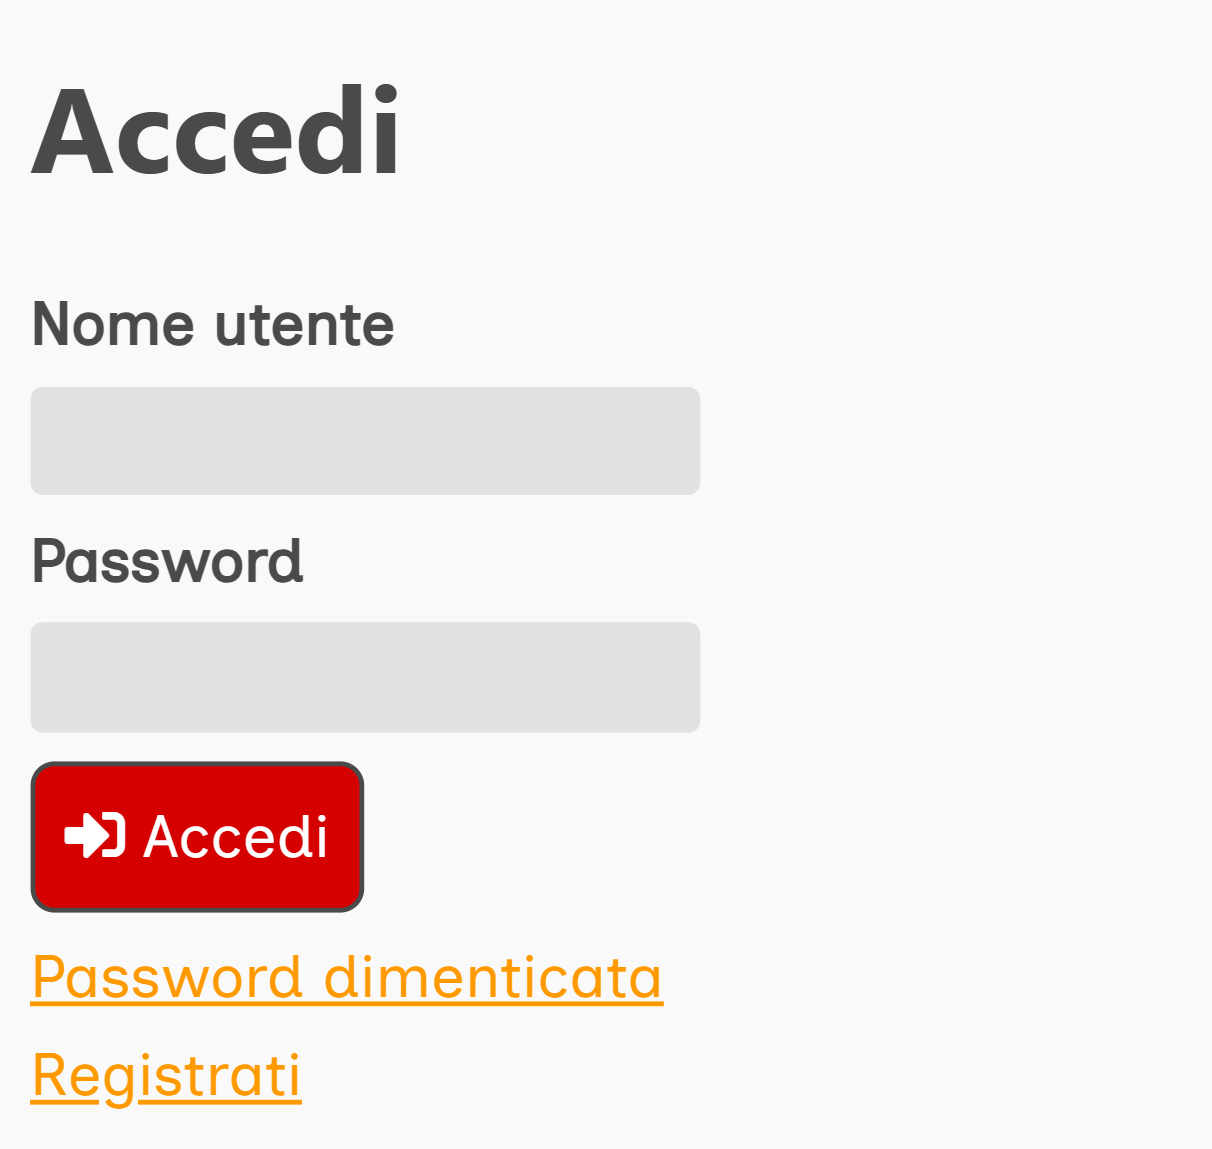
\includegraphics[width=0.45\textwidth]{assets/it/signin.png}
        \caption{Pagina di accesso}
    \end{figure}

    Una volta entrati, avrete accesso alla \emph{homepage}.

    \begin{figure}[H]
        \centering
        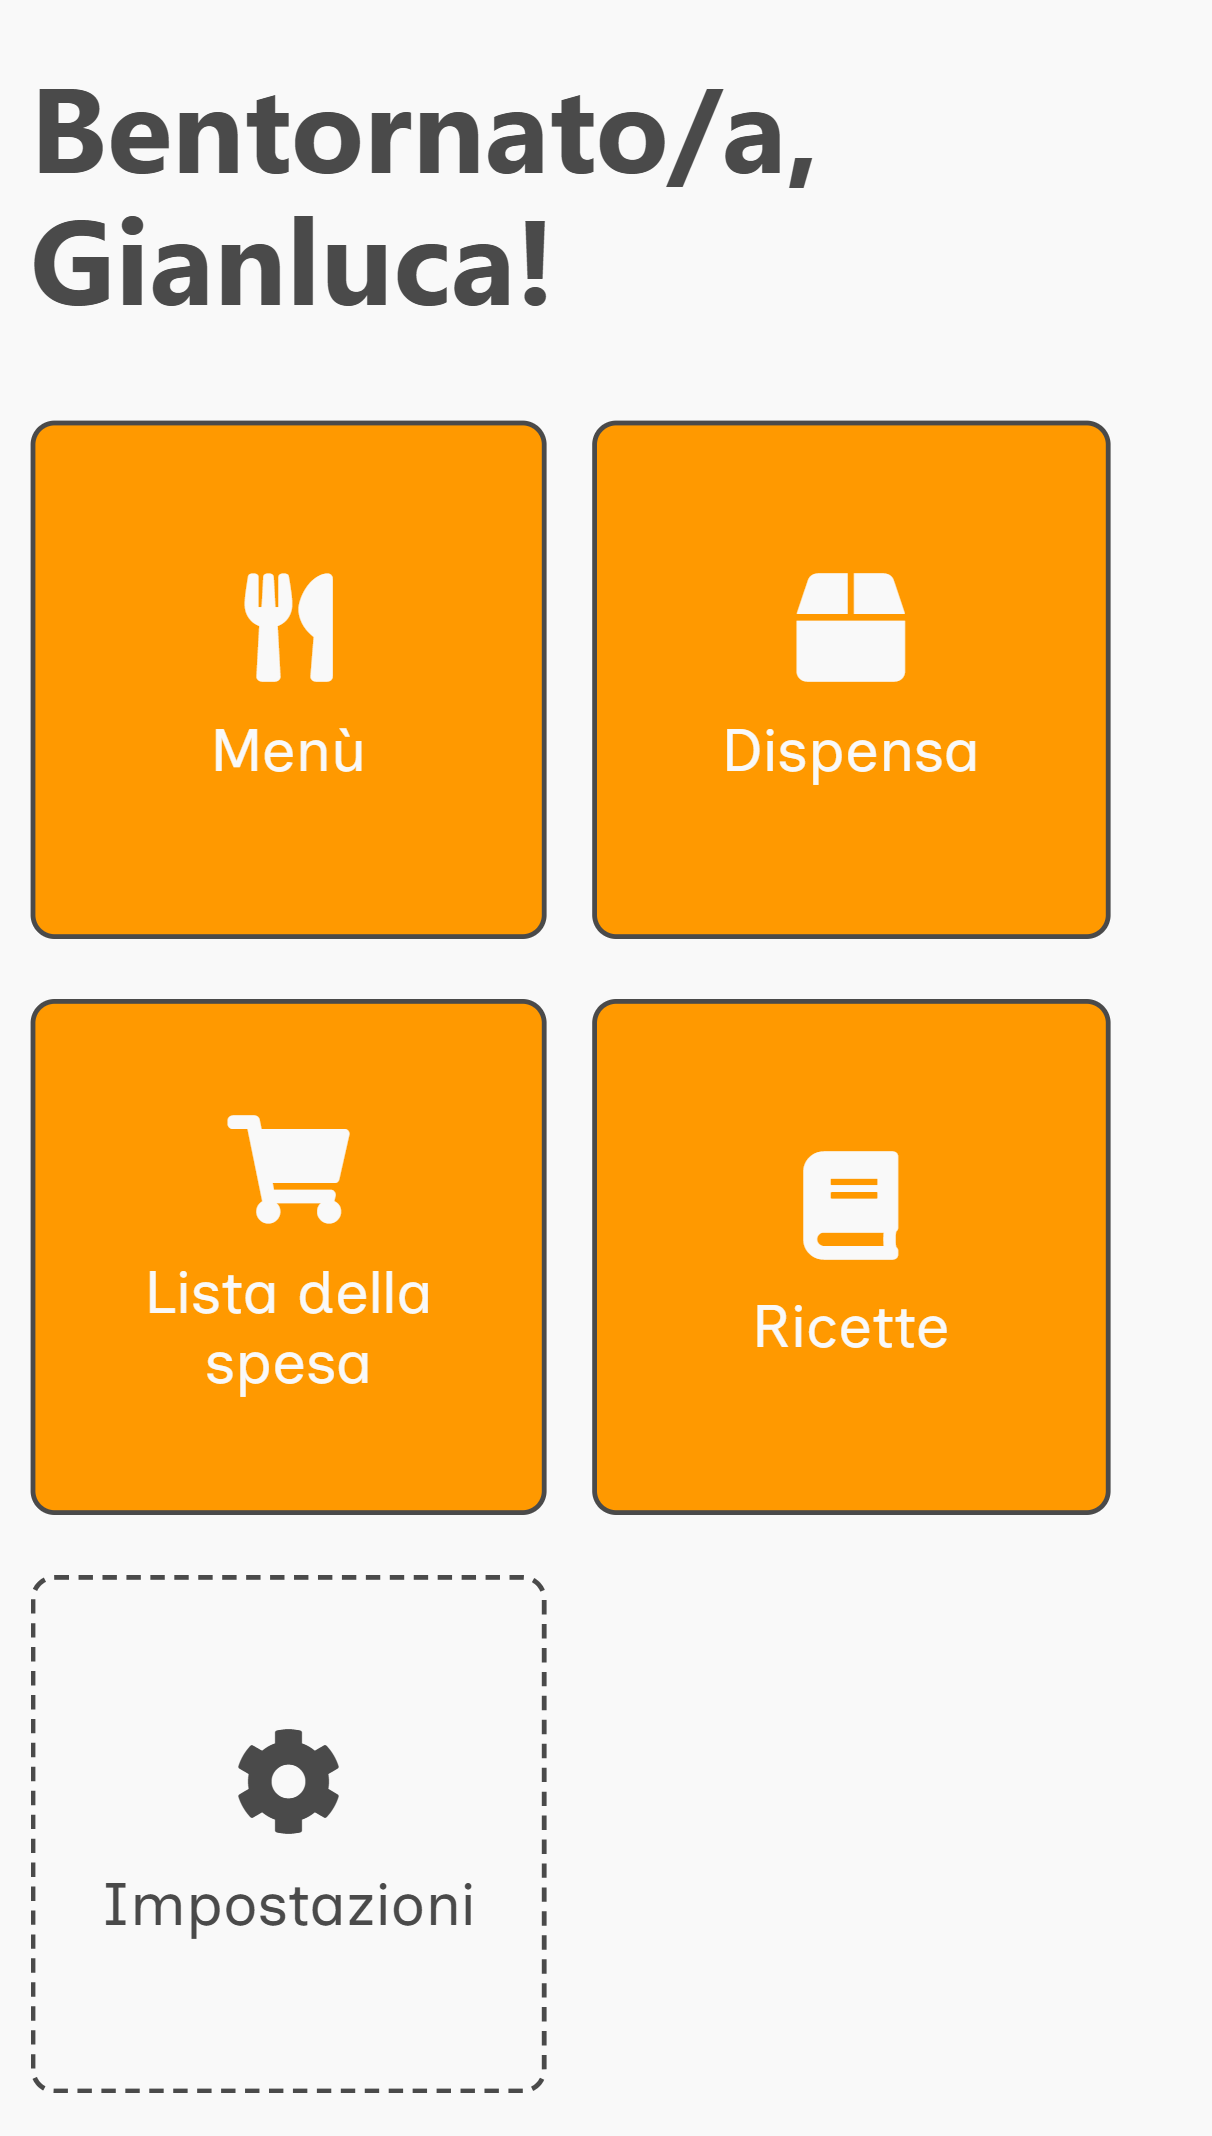
\includegraphics[width=0.45\textwidth]{assets/it/home.png}
        \caption{Pagina principale}
    \end{figure}

    \section{Impostazioni}

    Nelle impostazioni, oltre ad il tasto per disconnettervi, troverete anche dei bottoni per cambiare nome utente, email e password, eliminare
    l'account in maniera definitiva, e inoltre cambiare la lingua delle email. 

    Quest'ultima è un'impostazione a parte rispetto alla lingua di visualizzazione del sito, dunque potreste decidere di impostarla ad una lingua
    diversa.



    \chapter{Menù}

    I menù sono formati da un nome e 14 pasti, due al giorno per una settimana.

    \section{Panoramica}

    Dalla panoramica dei menù potrete vedere tutti i menù creati in precedenza (in ordine cronologico) e crearne di nuovi.

    \begin{figure}[H]
        \centering
        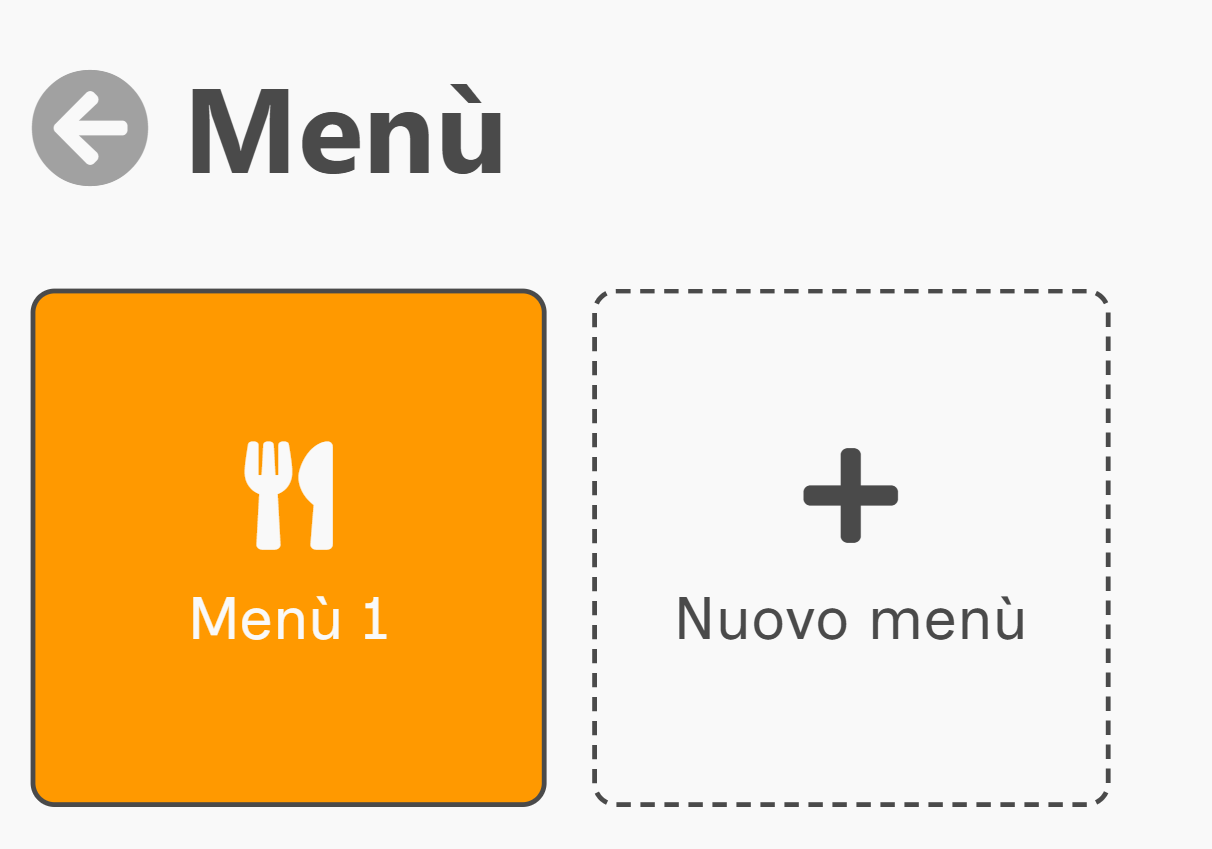
\includegraphics[width=0.45\textwidth]{assets/it/menus.png}
        \caption{Panoramica dei menù salvati}
    \end{figure}

    Una volta cliccato un menù potrete vederne il contenuto, e all'occorrenza modificarlo o duplicarlo. Per eliminarlo basterà cliccare
    prima il tasto \emph{Modifica}.

    \begin{figure}[H]
        \centering
        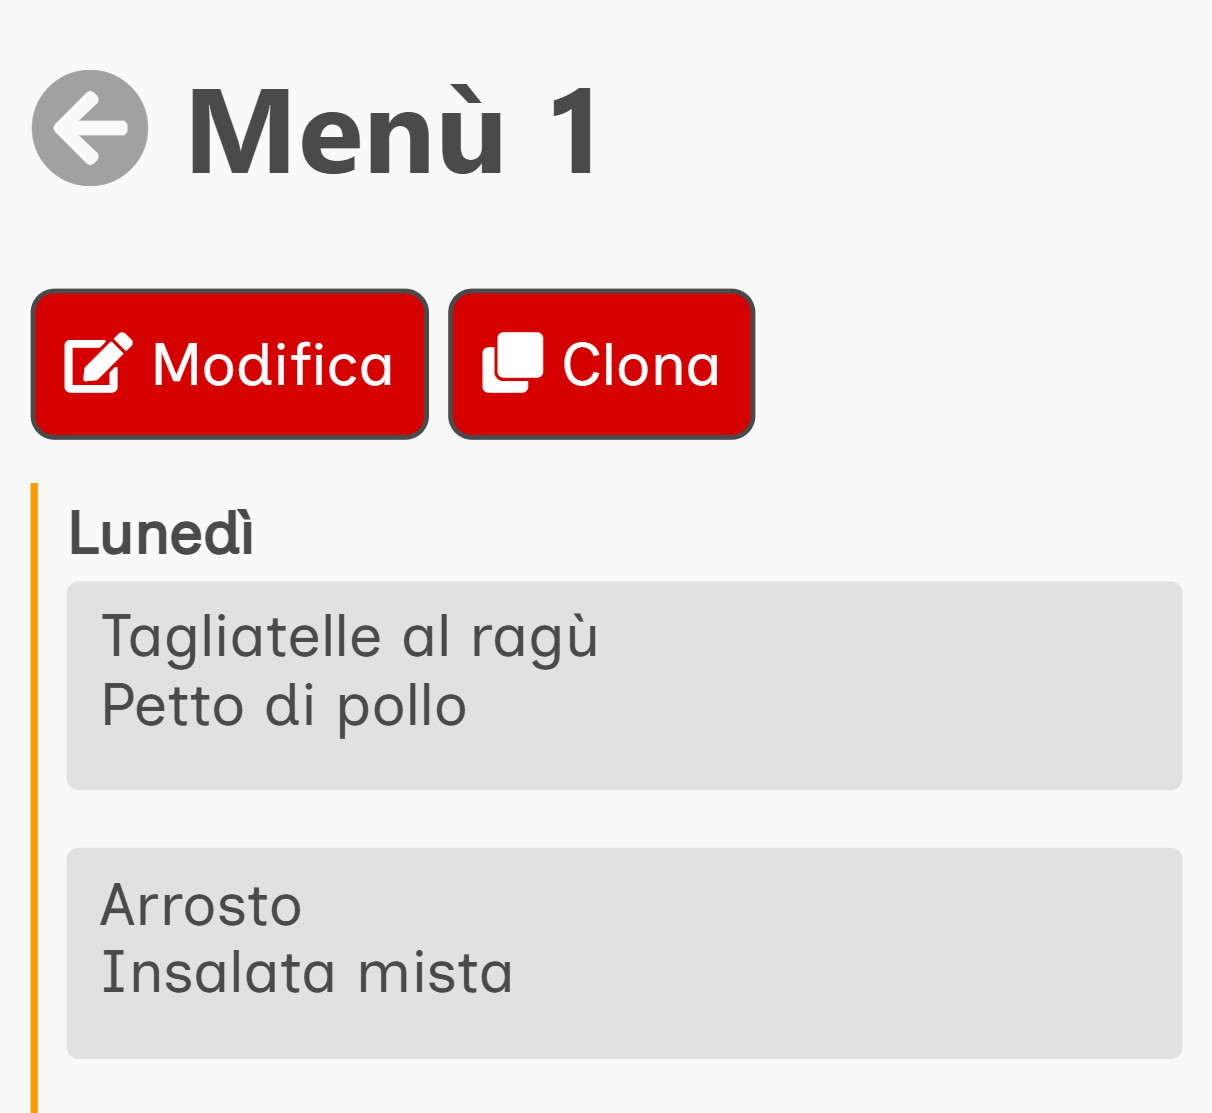
\includegraphics[width=0.45\textwidth]{assets/it/menu.png}
        \caption{Un esempio di menù}
    \end{figure}



    \chapter{Dispensa}

    Questa è la sezione più articolata di CucinAssistant.

    All'interno della dispensa, divisi in sezioni, potete inserire degli articoli: cose che avete nella vostra cucina, con un nome, una data di
    scadenza (opzionale) e una quantità\footnote{Anche non intera, come 1,5.} (opzionale).

    \section{Sezioni}

    Come detto in precedenza, gli articoli possono essere raggruppati in sezioni, che potete vedere cliccando sul pulsante \emph{Dispensa} nella
    pagina principale.

    \begin{figure}[H]
        \centering
        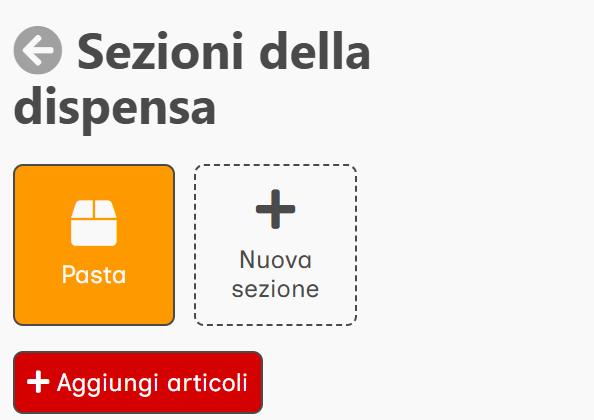
\includegraphics[width=0.45\textwidth]{assets/it/sections.png}
        \caption{Panoramica della dispensa}
    \end{figure}

    Potete creare nuove sezioni con il pulsante apposito; per modificare (o eliminare) una sezione dovrete aprirla e cliccare sul pulsante
    \emph{Modifica sezione}.

    \section{Articoli}

    Per vedere gli articoli in una sezione basterà cliccarla (e, in caso, cercare per nome).

    Gli articoli sono ordinati in base alla loro data di scadenza; gli articoli scaduti sono contrassegnati da una banda rossa a sinistra, invece
    della solita banda arancione.

    \begin{figure}[H]
        \centering
        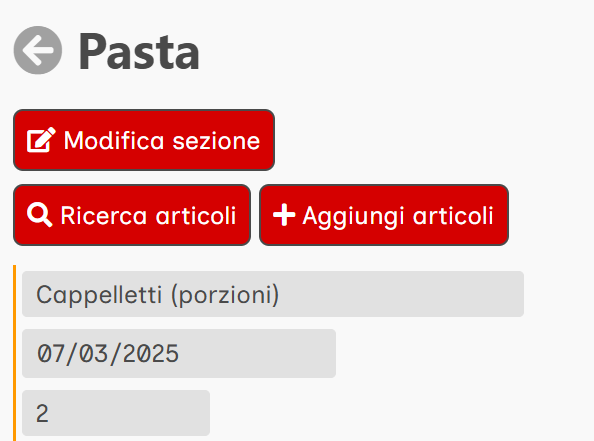
\includegraphics[width=0.45\textwidth]{assets/it/articles.png}
        \caption{Una sezione di esempio}
    \end{figure}

    Potete aggiungere articoli sia dall'interno della sezione che dall'esterno di essa; nell'ultimo caso, per ogni articolo è necessario specificare
    la sezione in cui deve essere salvato.

    Ricordate che un articolo è identificato dal nome e dalla data di scadenza, quindi se proverete ad aggiungere un articolo che avete già nella
    dispensa, CucinAssistant sommerà le quantità e non creerà duplicati; nel caso in cui la data di scadenza non coincida, verrà creato un nuovo
    articolo.

    \section{Modifica di articoli}

    Per modificare un articolo dovete cliccare su di esso. Fatto ciò, questo verrà mostrato con due frecce (o bottoni vuoti) e un bottone
    \emph{Elimina}; i bottoni con le frecce servono per scorrere tra gli articoli nella sezione, nello stesso ordine della lista a vista.

    Se volete eliminare un articolo, potete semplicemente cliccare sul bottone; se volete modificarlo, potete farlo direttamente: una volta che
    qualcosa è stato modificato, i tre bottoni verranno nascosti e verranno mostrati i bottoni \emph{Salva} e \emph{Annulla}, in modo da confermare
    (o annullare) le modifiche, per poi procedere con gli altri articoli. Cambiando la data di scadenza di un articolo è possibile che l'ordine cambi: in questo caso sarete reindirizzati alla lista.

    \begin{figure}[H]
        \centering
        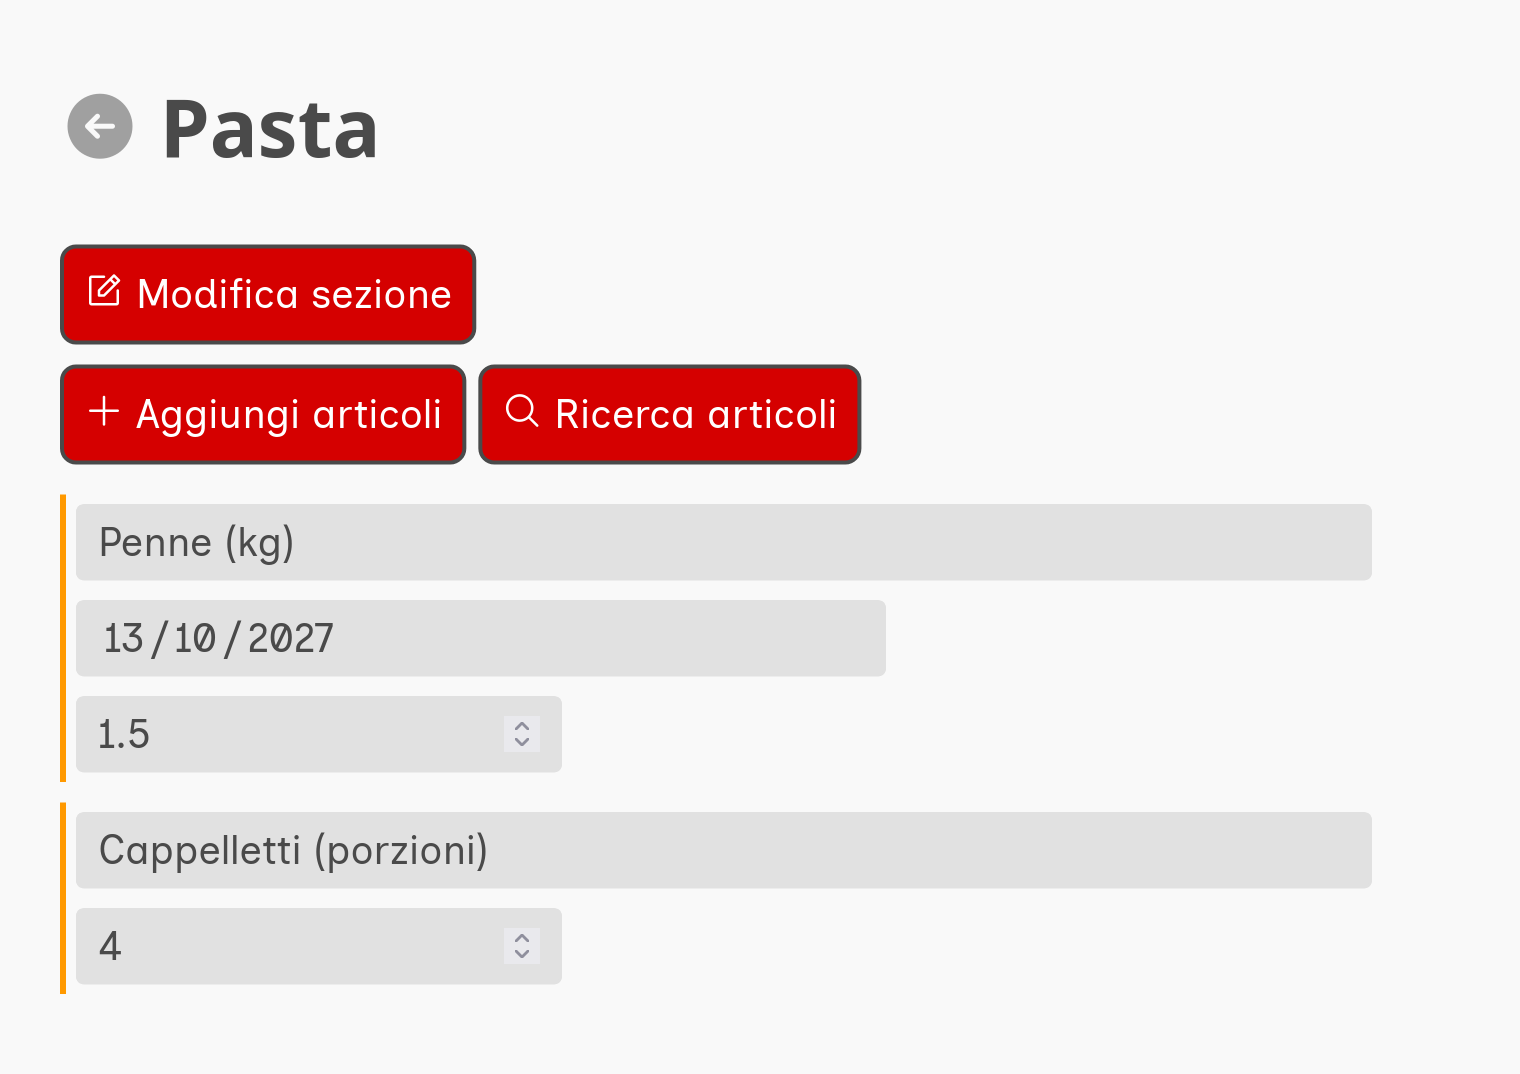
\includegraphics[width=0.45\textwidth]{assets/it/article.png}
        \caption{Un articolo di esempio che viene modificato, prima di ogni modifica}
    \end{figure}



    \chapter{Lista della spesa}

    È... la lista della spesa.

    \section{Panoramica}

    Una volta che avete aperto la lista, potrete vedere tutti gli elementi aggiunti.

    \begin{figure}[H]
        \centering
        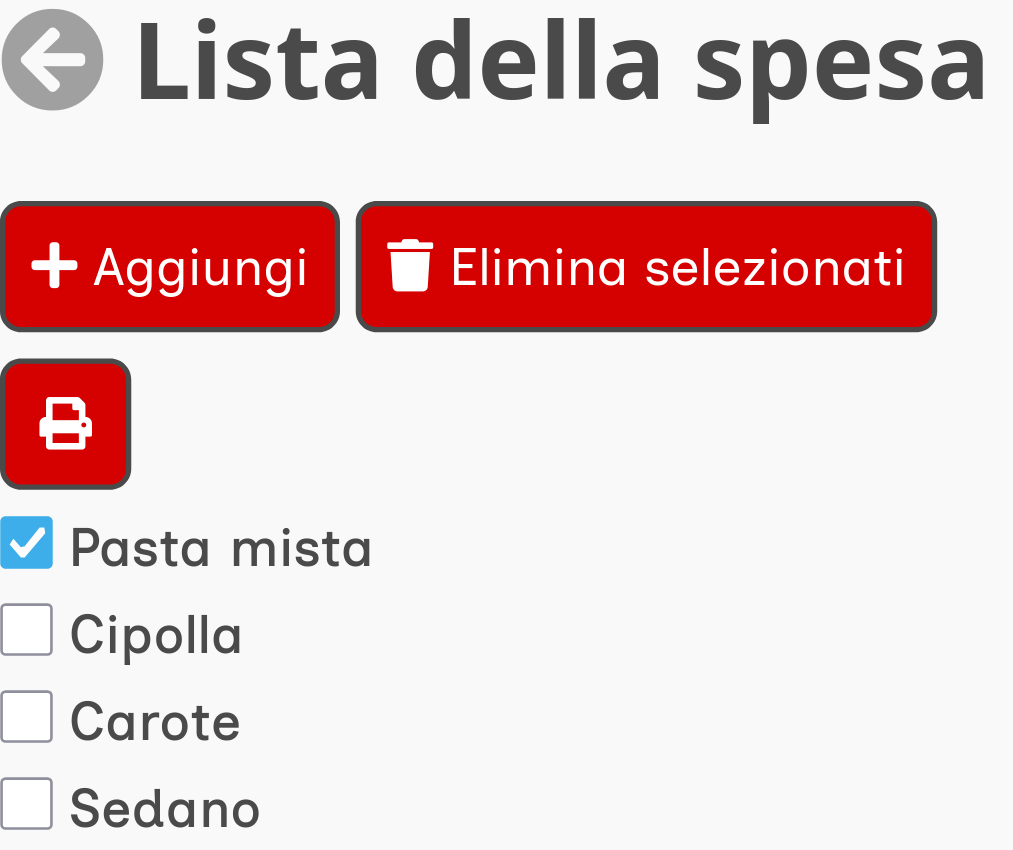
\includegraphics[width=0.45\textwidth]{assets/it/shopping_list.png}
        \caption{Una lista della spesa}
    \end{figure}

    Quando comprate qualcosa, cliccando sul quadrato a sinistra del nome potrete spuntare quell'elemento\footnote{Come tutto su CucinAssistant,
    questa cosa sarà visibile da tutti i dispositivi}, che rimarrà comunque nella lista; per eliminarlo potete cliccare sul tasto \emph{Elimina
    selezionati}.

    Per aggiungere nuovi elementi potete usare il pulsante \emph{Aggiungi elementi}; per modificarne uno basterà cliccare sul nome.



    \chapter{Recipes} \label{recipes}

    Una ricetta è composta da un nome (l'unica componente obbligatorio), una valutazione (da 0,5 a 5,0 stelle), una lista di ingredienti, un
    procedimento e delle note aggiuntive.

    \section{Overview}

    Cliccando il pulsante \emph{Recipes} potrete vedere tutte le ricette salvate, e un bottone per crearne di nuove.

    \begin{figure}[H]
        \centering
        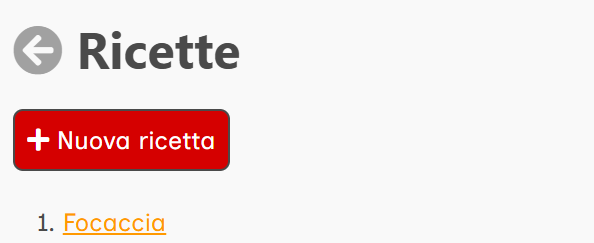
\includegraphics[width=0.45\textwidth]{assets/it/recipes.png}
        \caption{Una lista di ricette}
    \end{figure}

    Per vederne una in dettaglio basterà cliccarla, e vedrete tutte le sue componenti (tutte quelle che non sono vuote).

    \begin{figure}[H]
        \centering
        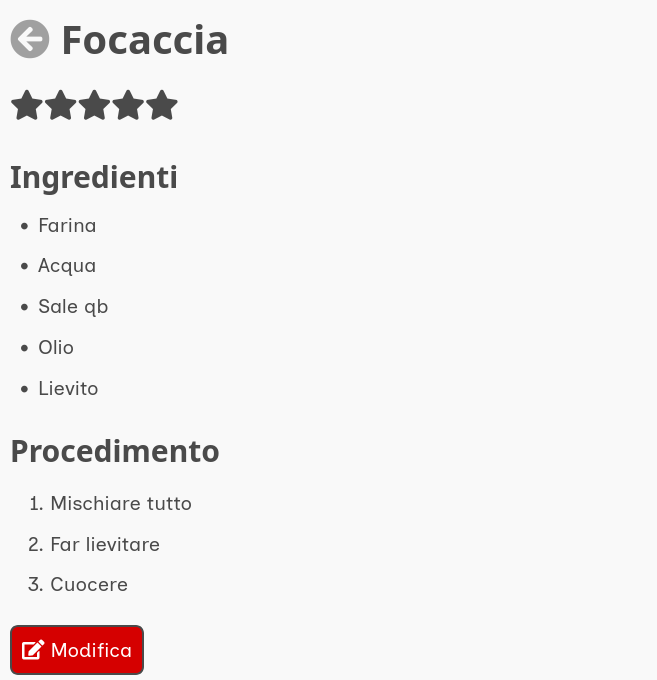
\includegraphics[width=0.45\textwidth]{assets/it/recipe.png}
        \caption{Una ricetta di esempio}
    \end{figure}

    Per modificarla o eliminarla potete cliccare sul pulsante \emph{Modifica}.

    Per nascondere le stelle potete impostarne il numero a 0. Quando scrivete gli ingredienti e il procedimento, ricordatevi di andare a capo per
    vederli formattati correttamente.
\end{document}
